\documentclass[12pt]{article}

\usepackage{amsthm}
\usepackage{graphicx}

\begin{document}

\theoremstyle{definition}
\newtheorem{definition}{Definition}[section]

\theoremstyle{remark}
\newtheorem*{remark}{Remark}
\newtheorem{theorem}{Theorem}[section]
\newtheorem{lemma}[theorem]{Lemma}

\section{On a special intersection graph of class 2}
Our interest here is to find a graph of class 2 with $\Delta = 3$ and $\omega = 2$. Moreover, we want to ask ourselves if such a graph can be an intersection graph
of squares, and an intersection graph of unit squares.\\
Let's take a look at the following graph:

\begin{figure}[h]
    \centering
    \caption{Graph $G$ used as a base.}
    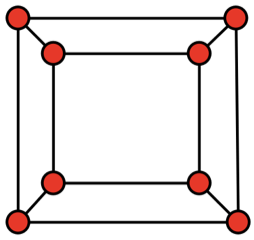
\includegraphics[scale=0.5]{tex_images/8cube.png}

\end{figure}

\begin{lemma}
    A graph obtained by replacing an edge of $G$ by a vertex of degree 2 is not 3-edge colorable.
\end{lemma}

\begin{proof}
    Notice that the previous embedding of $G$ is consisting of two rectangles, one inside the other, with edges linking the cornes. 
    Call $a, b, c, d$ the corners of the inner rectangle, and $A, B, C, D$ the corner of the outer rectangle.\\
    The edges we consider are the obvious $ab, bc, cd, da$ (same for capitals) and the $aA$ (same for other letters.).\\
    Then we obtain an other graph, $G^'$ by supressing $AB$, adding a vertex $O$, then adding two edges: $AO$ and $OB$.\\

    \begin{figure}[h]
        \centering
        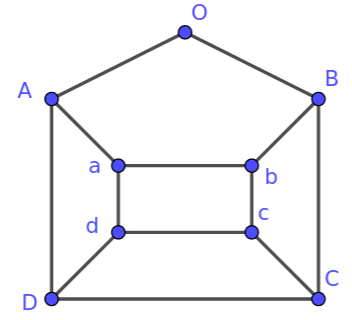
\includegraphics[scale=0.4]{tex_images/Gprime_uncolored.png}
    \end{figure}

    We start by coloring the 5-cycle $AOBba$. Without loss of generality, consider that a 3-coloring of it uses two times colors 1 and 2, and one time color 3. Consider the three following cases:
    \begin{itemize}
        \item 1. color 3 is on the $AO$ edge.
        \item 2. color 3 is on the $ab$ edge.
        \item 3. color 3 is on the $Aa$ edge. testestest
    \end{itemize}

    \textbf{\underline{case 1:}} \\
    Suppose $Aa$ is in color 1 and $AO$ is in 3.  . Then, by trying to use only 3 colors you end up with, in the following order: \\
    $ad$ 3; $bc$ 3; $BC$ 3; $AD$ 2; $Dd$ 1. Then you are forced to color $DC$ in a 4th color. \\

    \begin{figure}[h]
        \centering
        \caption{Case 1: we end up needing a 4th color.}
        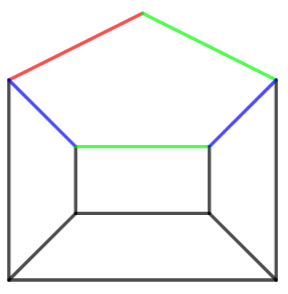
\includegraphics[scale=0.3]{tex_images/case_1_1.png}
        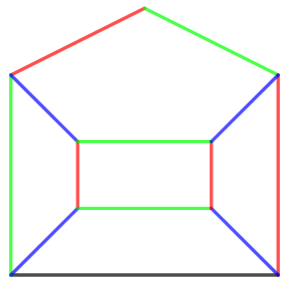
\includegraphics[scale=0.3]{tex_images/case_1_2.png}
    \end{figure}

    \textbf{\underline{case 2:}} \\
    Suppose $Aa$ is in color 1. Then you must color in the following order: \\
    $ad$ 2; $AD$ 3; $Dd$ 1; $dc$ 3; $bc$ 1; $cC$ 2. Then you have to use a 4th color for $Dd$.\\

    \textbf{\underline{case 3:}} \\
    Suppose $Aa$ is in 3 and $ab$ is in 1. The coloring order is:\\
    $ad$ 2; $bc$ 3; $dc$ 1; $Dd$ 3; $Cc$ 2; $DC$ 1. Then a 4th color is necessary for $BC$ and $AD$. 

    
\end{proof}


\newpage

\subsection{Case of squares intersection graph}
\begin{lemma}
    $G^'$ can be the intersection graph of axis parralel squares.
\end{lemma}
Observe an example of such a graph:
\begin{figure}[h]
    \centering
    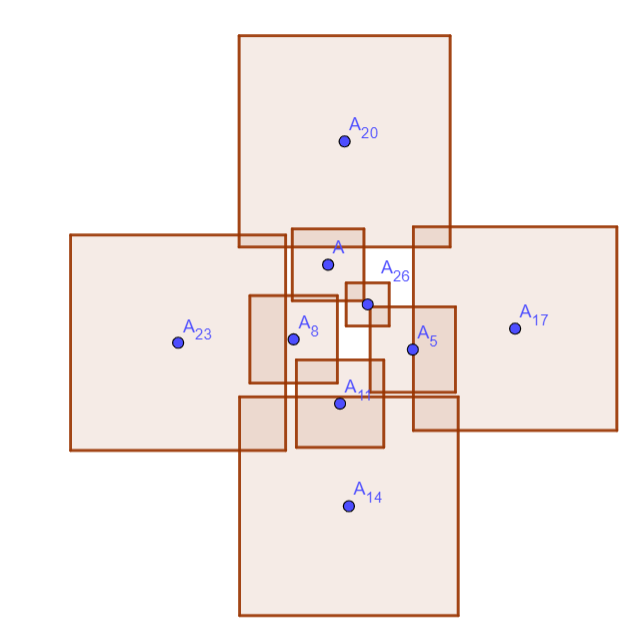
\includegraphics[scale=0.4]{tex_images/8cube+_as_squares.png}        
\end{figure}



\subsection{Case of unit squares intersection graph}

\begin{definition}[direction of an intersection for unit squares]
    We say that a square $a$ intersect $b$ in the direction "UL" if the upper-left corner of $a$ lies in $b$. 
    Consequently, it would means $b$ intersect $a$ in the "DR" direction. There is 4 different directions: "UL", "UR", "DR", "DL"
\end{definition}

\begin{remark}
    Right now, we will suppose that a square $a$ can't intersect a square $b$ in two adjacent directions (see definition 1.2) at the same time. 
    Later we will prove that in the case of our problem, this is not possible: see lemma 1.5.
\end{remark}

\begin{lemma}
    If $a$ intersect $b$ in a direction and $a$ intersect $c$ in the same direction, then $b$ and $c$ must intersect. 
\end{lemma}

\begin{remark}
    Thus, if $a$ intersect $b$ in a direction, and $a$ intersect $c$; such that $b$ and $c$ do not intersect, then the intersection of $a$ and $c$ must be in a different direction.
\end{remark}

\begin{lemma}
    Let $a$ and $b$ two unit squares with affixes respectively $z_a$ and $z_b$ and $p_x, p_y$ the projections on axis $x, y$. Then:
    \begin{center}
        $a \cap b = \emptyset \Leftrightarrow (|p_x(z_a) - p_x(z_b)| > 1)$ or $(|p_y(z_a) - p_y(z_b)| >1)$

    \end{center}
\end{lemma}


\begin{proof}
    Trivial.
\end{proof}

\begin{definition}[adjacent directions]
    $a$ intersect $b$ and $c$ in distinct adjacent directions if the corners of $a$ that are inside $b$ and $c$ lies on an edge of $a$. 
    For instance, UR and DL are not adjacent directions.    
\end{definition}

\begin{lemma}
    If $a$ intersect $b$ in direction UL and $c$ in directions UR and DL at the same time, then:
    \begin{center}
        $\forall d$ such that $d \cap b \ne \emptyset$ and $d \cap c \ne \emptyset \Rightarrow d \cap a \ne \emptyset$
    \end{center} 
\end{lemma}

\begin{proof}
    As $a$ and $c$ share $a$'s upper and down right corners, the only possibility for $d$ and $c$ to intersect without $d$ intersection $a$
    would be that $c$ interest $d$ in direction UL or DL. Applying lemma 1.4 on $d$ and $c$ on axis $x$ and noticing that $p_x(z_c) < p_x(z_d)$ would give us
    that $p_x(z_b) < 1 + p_x(z_d)$, ie $d \cap b = \emptyset$.
\end{proof}

\begin{remark}
    This implies that in an intersection graph of unit squares that is a $C_4$, we can't find two squares with one having two of it's corners inside the other.  
\end{remark}



\begin{lemma}
    Let $G$ be $C_4$, an intersection graph of unit squares. Then; $\forall v \in V(G)$, $v$ intersects it's neighbours in adjacent directions.
\end{lemma}



\begin{proof}
    Let $p_x$ and $p_y$ the projections on respectively $x$ and $y$ axis.\\
    Let $a, b, c$ and $d$ be unit squares such that their corresponding intersection graph is $C_4$. Without loss of generality, suppose 
    that $a$ intersect $b$ in direction UR and $a$ intersect $d$ in direction DL. \\ 
    Call $z_a, z_b, z_c$ and $z_d$ the affixes of the center of the squares.
    \begin{figure}[h]
        \centering
        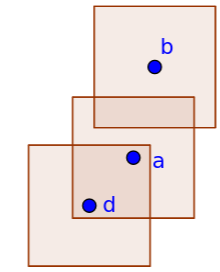
\includegraphics[scale=0.4]{tex_images/proof_1_4_1.png}
    \end{figure}
    \\
    If $c$ intersect $d$ in direction DL, then $a, c$ and $d$ would share a common point in the upper right corner of $d$, contradicting the fact we have $C_4$.\\
    Suppose $c$ intersect $d$ in a direction different than DL such that $a$ and $c$ share no common point; then $c \cap b = \emptyset$, and we shall prove this using projections.
    As $a$ and $c$ share no commont point, in at least one of the projections, we must have an empty intersection. Call it $p$.
    Thus, we have $p(z_c) < 1 + p(z_a)$.
    as $a$ intersect $b$ in UR direction, then $p_x(z_a) < p_x(z_b)$ and $p_y(z_a) < p_y(z_b)$.
    By transitivity; we must have $p(z_c) < 1+ p(z_b)$; or, in other words; $c \cap b = \emptyset$.
\end{proof}

\begin{theorem}
    $G^'$ can't be a intersection graph of unit squares.
\end{theorem}

\begin{proof}
    We will actually prove that a subgraph of $G^'$ can't be done with unit squares. Let $G^{''}:=G'[U]$ with $U := \{a, b, d, c, C, D, A\}$
    The proof is done by trying to construct the squares according to the edges of $G''$.\\
    First, place $d$. It belongs to three cycles of size 4 at the same time through it's three neighbours: $a, c$ and $D$. Suppose, without loss of generality,
    that $d$ intersect $a$ in direction UL; then $d$ must intersect $D$ in direction either DL or UR in order to complete the cycle $daAD$. For the same reason,
    $d$ must intersect $c$ in direction either DL or UR to complete $dcCD$. Thus, completing the cycle $abcd$ becomes impossible as $d$ is intersecting $a$ and $c$
    in non-adjacent directions. 
\end{proof}



\end{document}